\section{Trigger \label{sec:trigger}}
All events used in the analyses are required to be triggered by one of three algorithms. The algorithms require a high momentum track to be found online
and/or missing transverse energy, PFMET, as calculated by the particle flow algorithm~\cite{CMS:2010xta}. 

The particle flow algorithm attempts
to reconstruct all particles in an event, then calculates PFMET as the magnitude of the negative vector sum of the transverse momenta of the particles. 
As the proton-proton collision occurs
at rest in the transverse plane, PFMET is meant to represent the vector sum of all particles not found by the particle flow algorithm. For most CMS analyses, PFMET is created
by either the limited detector response in finding all tracks in an event and determining their momentum or from neutral particles in the event which leave no signals
in the detector. These neutral particles could be neutrinos from the SM or new neutral particles created in a BSM theory such as supersymmetry. 

For HSCP,
PFMET often arises because of details of the particle flow algorithm. The algorithm assumes SM particles and rejects tracks that do not conform to the properties expected
of a SM particle. Two types of possible HSCP tracks are rejected by the algorithm. 

The first type is tracks reconstructed only in the muon system. The only charged SM particles that
are expected to reach the muon system are muons. As muons should have a matching track in the inner tracker, particle flow rejects tracks found only in the
muon system. HSCP produced neutral then acquiring charge by interacting with the calorimeter
would only have a track in the muon system and as such would not be included in the PFMET calculation. 

The second type is tracks produced charged but becoming neutral as they propagate through CMS.
The particle flow algorithm rejects tracks reconstructed only in the inner tracker that have a track $p_T$ much larger
than the associated energy deposited in the calorimeter as this indicates the track has been misreconstructed.
As an HSCP only deposits approximately 10~GeV of energy in the calorimeter and normally has $>$ 100~GeV of momentum, HSCP neutral in the muon system will likely be rejected. 

These two effects lead to PFMET in HSCP events to be roughly equal to the vector sum of any $R$--hadrons neutral in
either the muon system or the inner tracker, less however much energy they deposit in the calorimeter. This effect can be seen in Figures~\ref{fig:SystPtTrigger} 
and~\ref{fig:SystPtTriggerN} which compare the di-HSCP system with online PFMET in events with at least 150~GeV of online PFMET.

\begin{figure}
  \begin{center}
      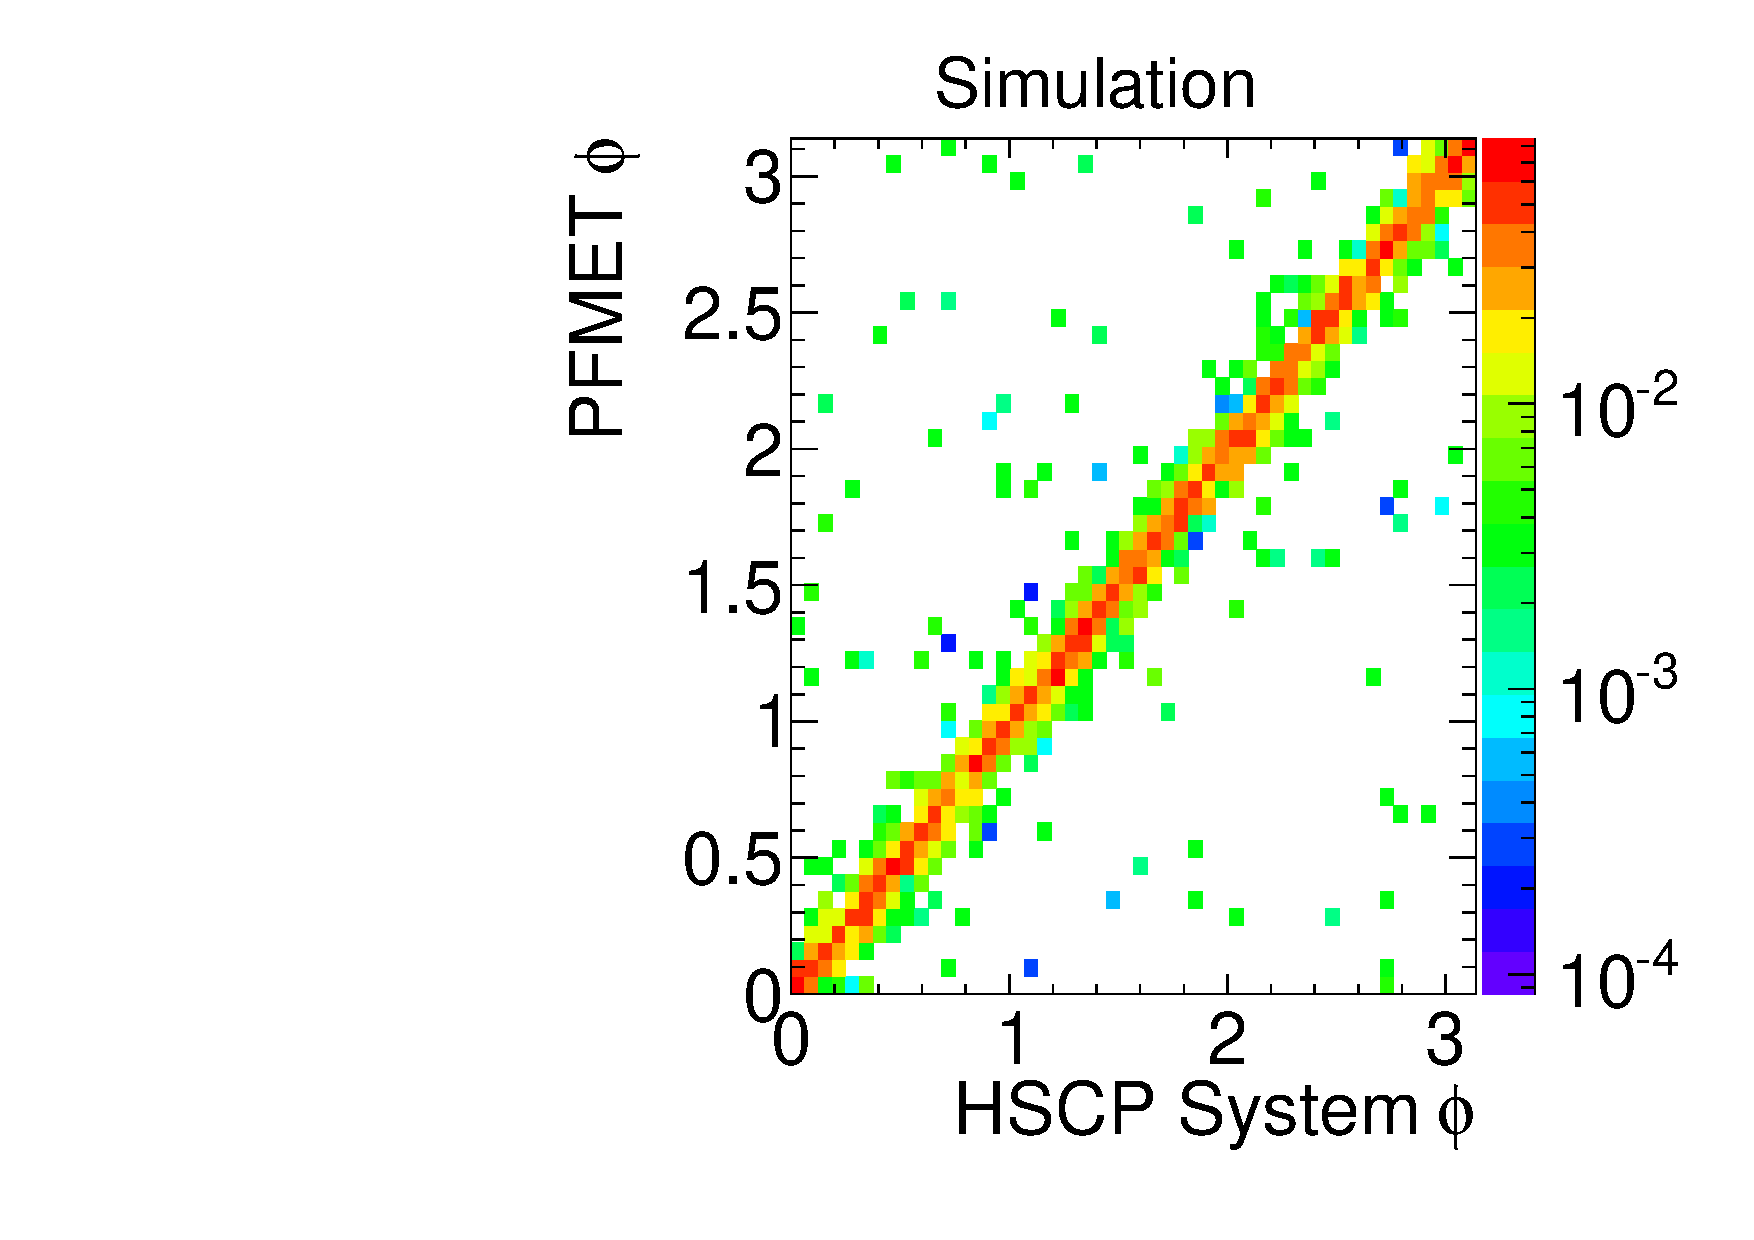
\includegraphics[clip=true, trim=0.0cm 0cm 3.0cm 0cm, width=0.44\textwidth]{figures/search/Gluino_8TeV_M1200_f100SystPhiMET}
      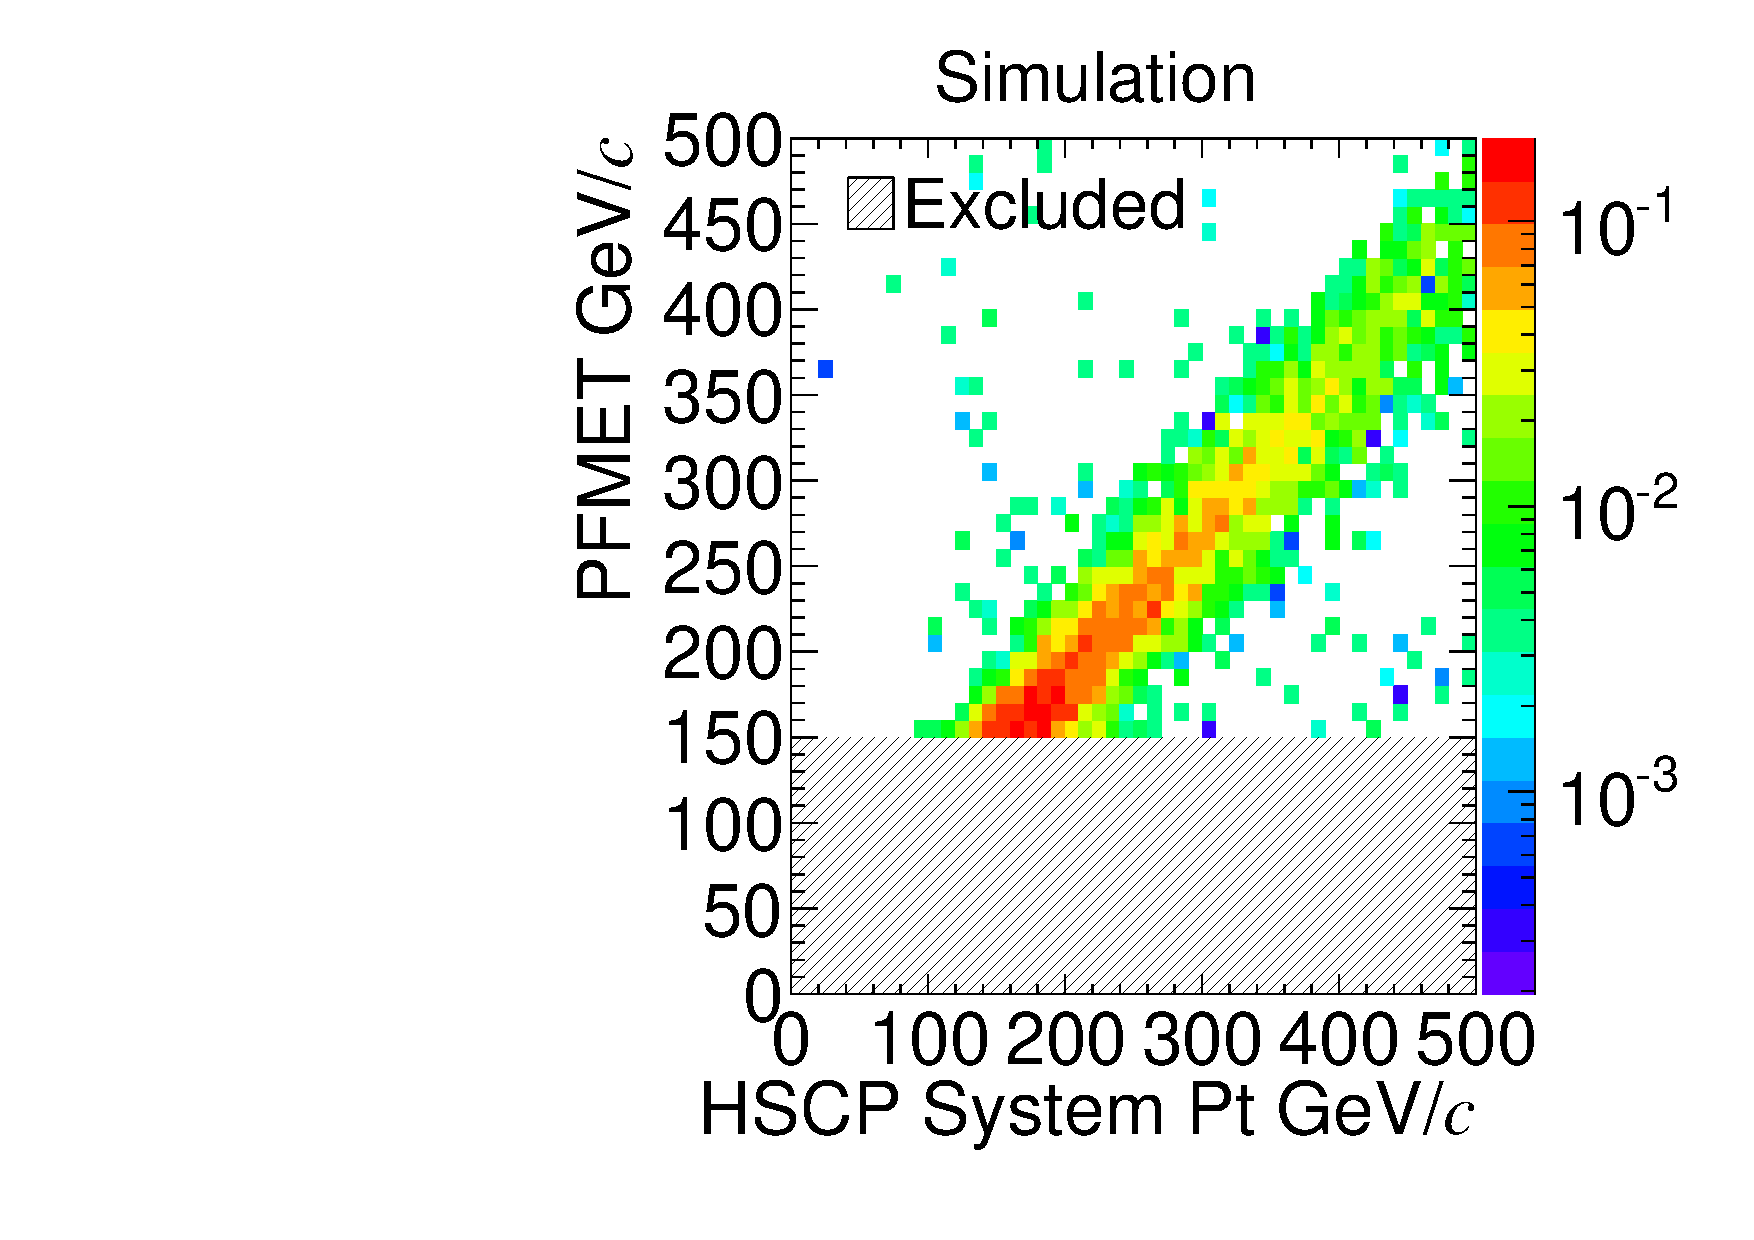
\includegraphics[clip=true, trim=0.0cm 0cm 3.0cm 0cm, width=0.44\textwidth]{figures/search/Gluino_8TeV_M1200_f100SystPtMET} \\
      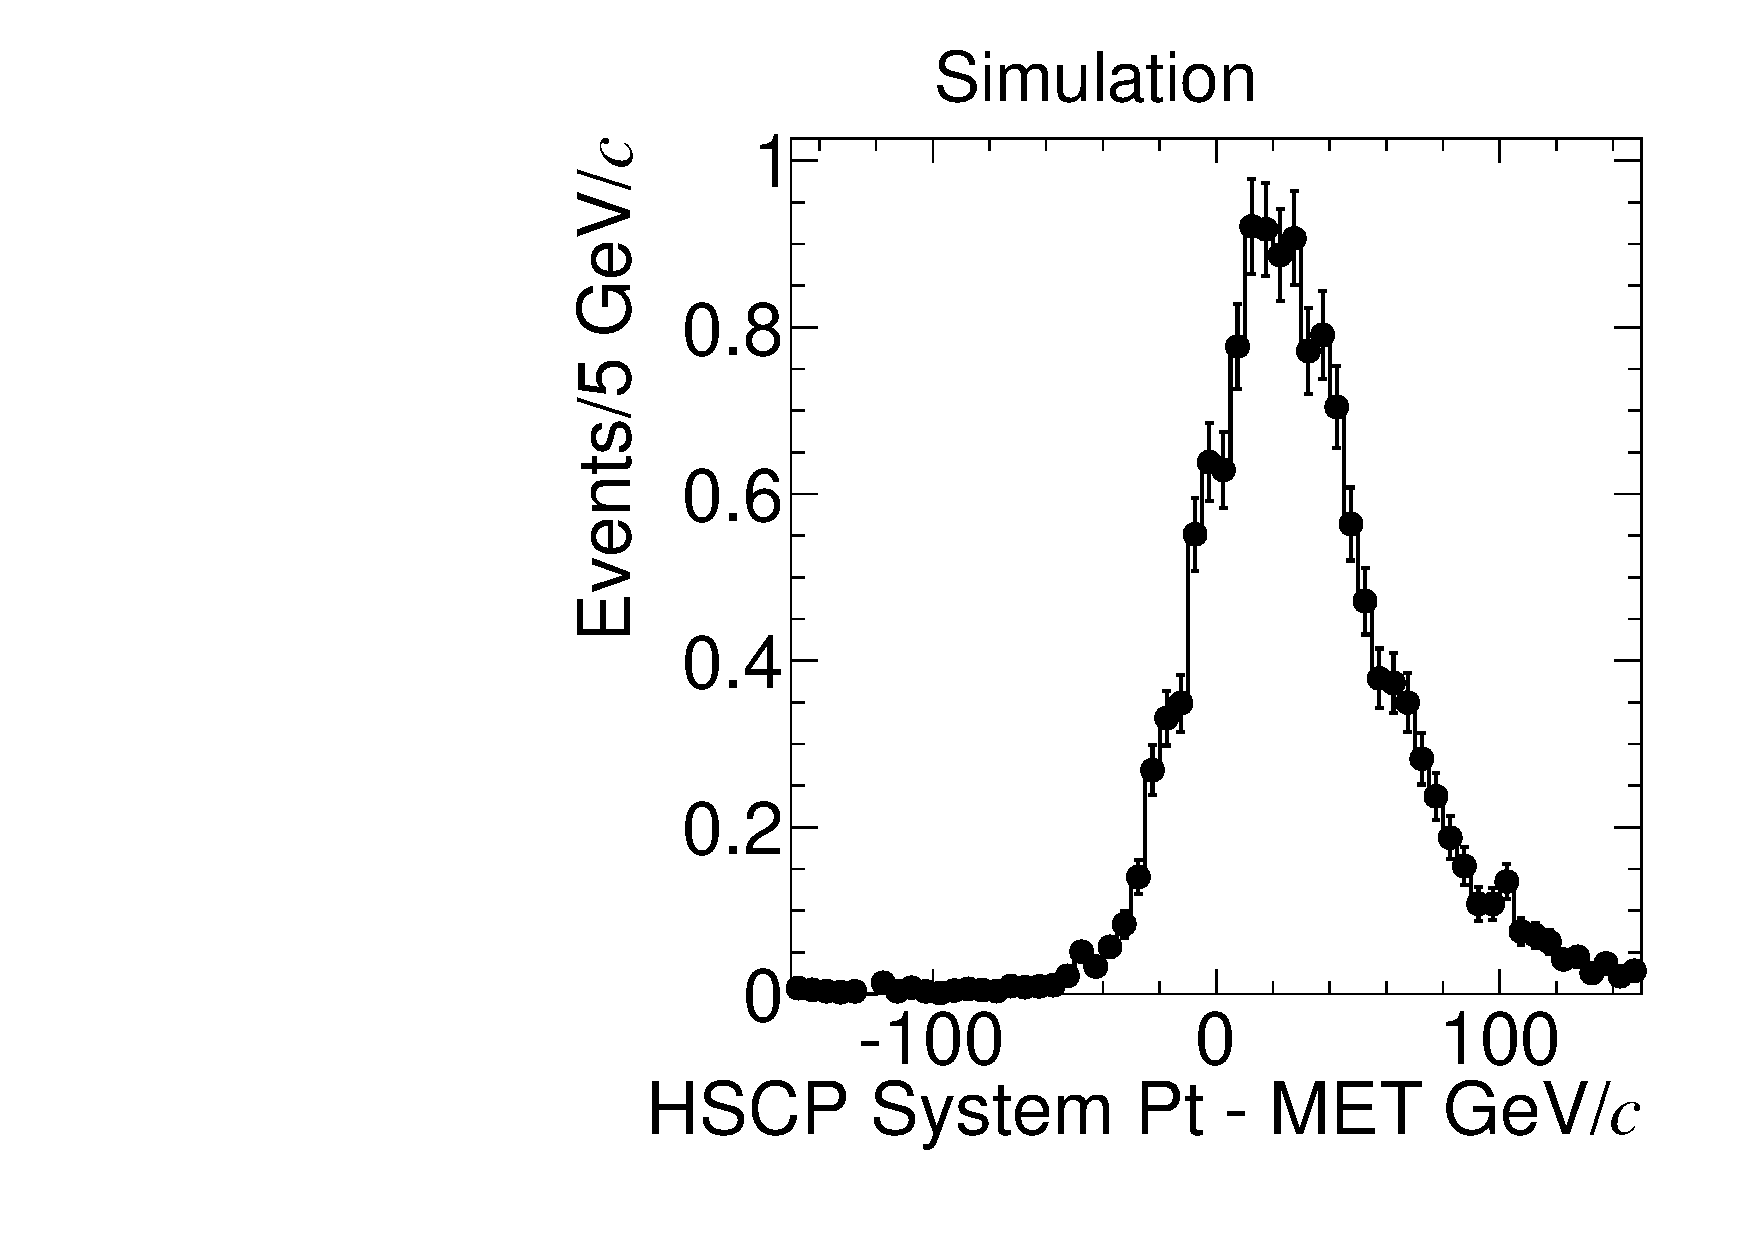
\includegraphics[clip=true, trim=0.0cm 0cm 3.0cm 0cm, width=0.44\textwidth]{figures/search/Gluino_8TeV_M1200_f100SystPtDiffMET}
      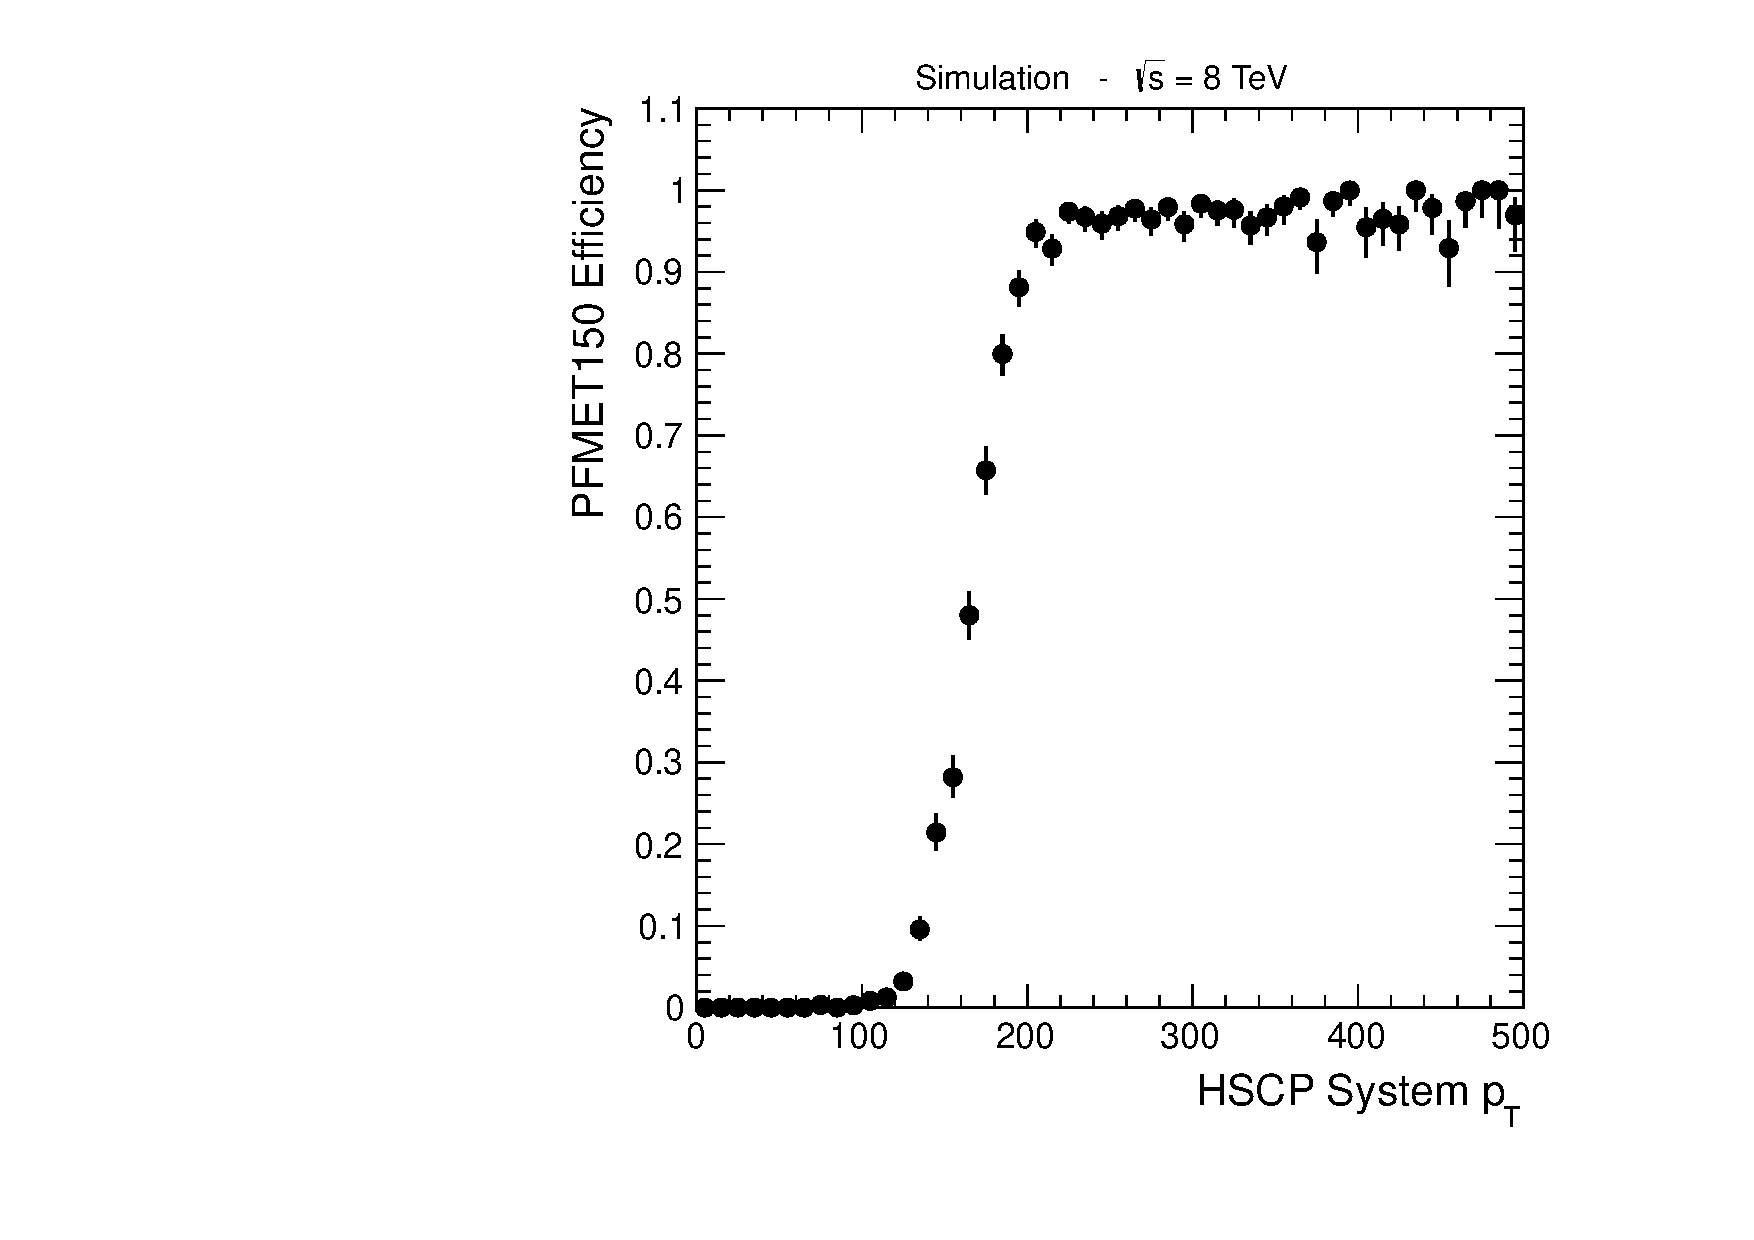
\includegraphics[clip=true, trim=0.0cm 0cm 3.0cm 0cm, width=0.44\textwidth]{figures/search/Gluino_8TeV_M1200_f100SystPtEff}
      \caption[Comparison of di-HSCP system $\phi$ and \pt\ with online PFMET for a 1200~GeV 
Gluino $f=1.0$ sample in events with at least 150~GeV of online PFMET.]
        {Comparison of di-HSCP system with online PFMET for a 1200~GeV Gluino $f=1.0$ sample in events with at least 150~GeV of online PFMET. 
         Top Left: Online PFMET $\phi$ versus di-HSCP system $\phi.$ Top Right: Online PFMET value versus di-HSCP system $p_T$. 
         Bottom Left: Difference between di-HSCP system $p_T$ and online PFMET value.
         Bottom Right: Probability to have online PFMET greater than 150~GeV versus di-HSCP system $p_T$.
        }
      \label{fig:SystPtTrigger}
  \end{center}
\end{figure}

\begin{figure}
  \begin{center}
      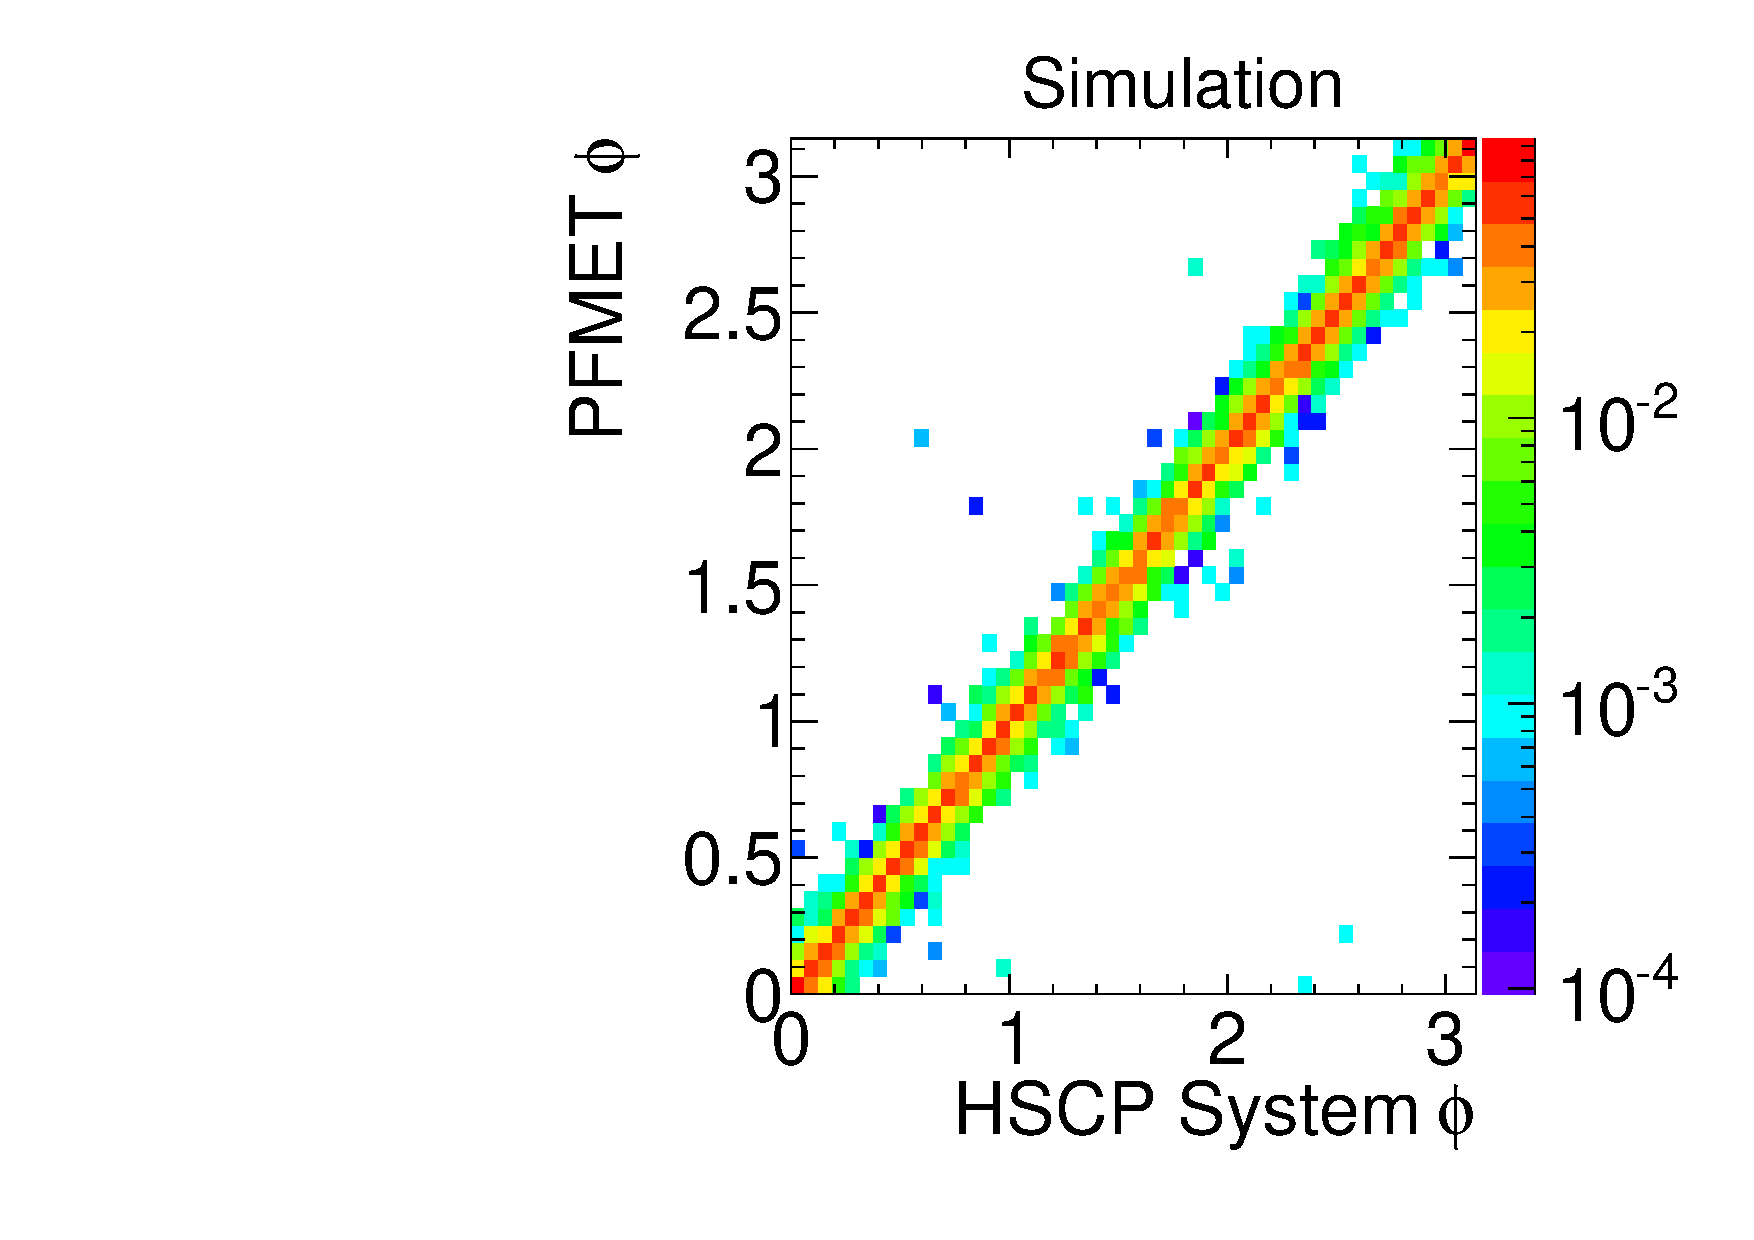
\includegraphics[clip=true, trim=0.0cm 0cm 3.0cm 0cm, width=0.44\textwidth]{figures/search/Gluino_8TeV_M1200N_f10SystPhiMET}
      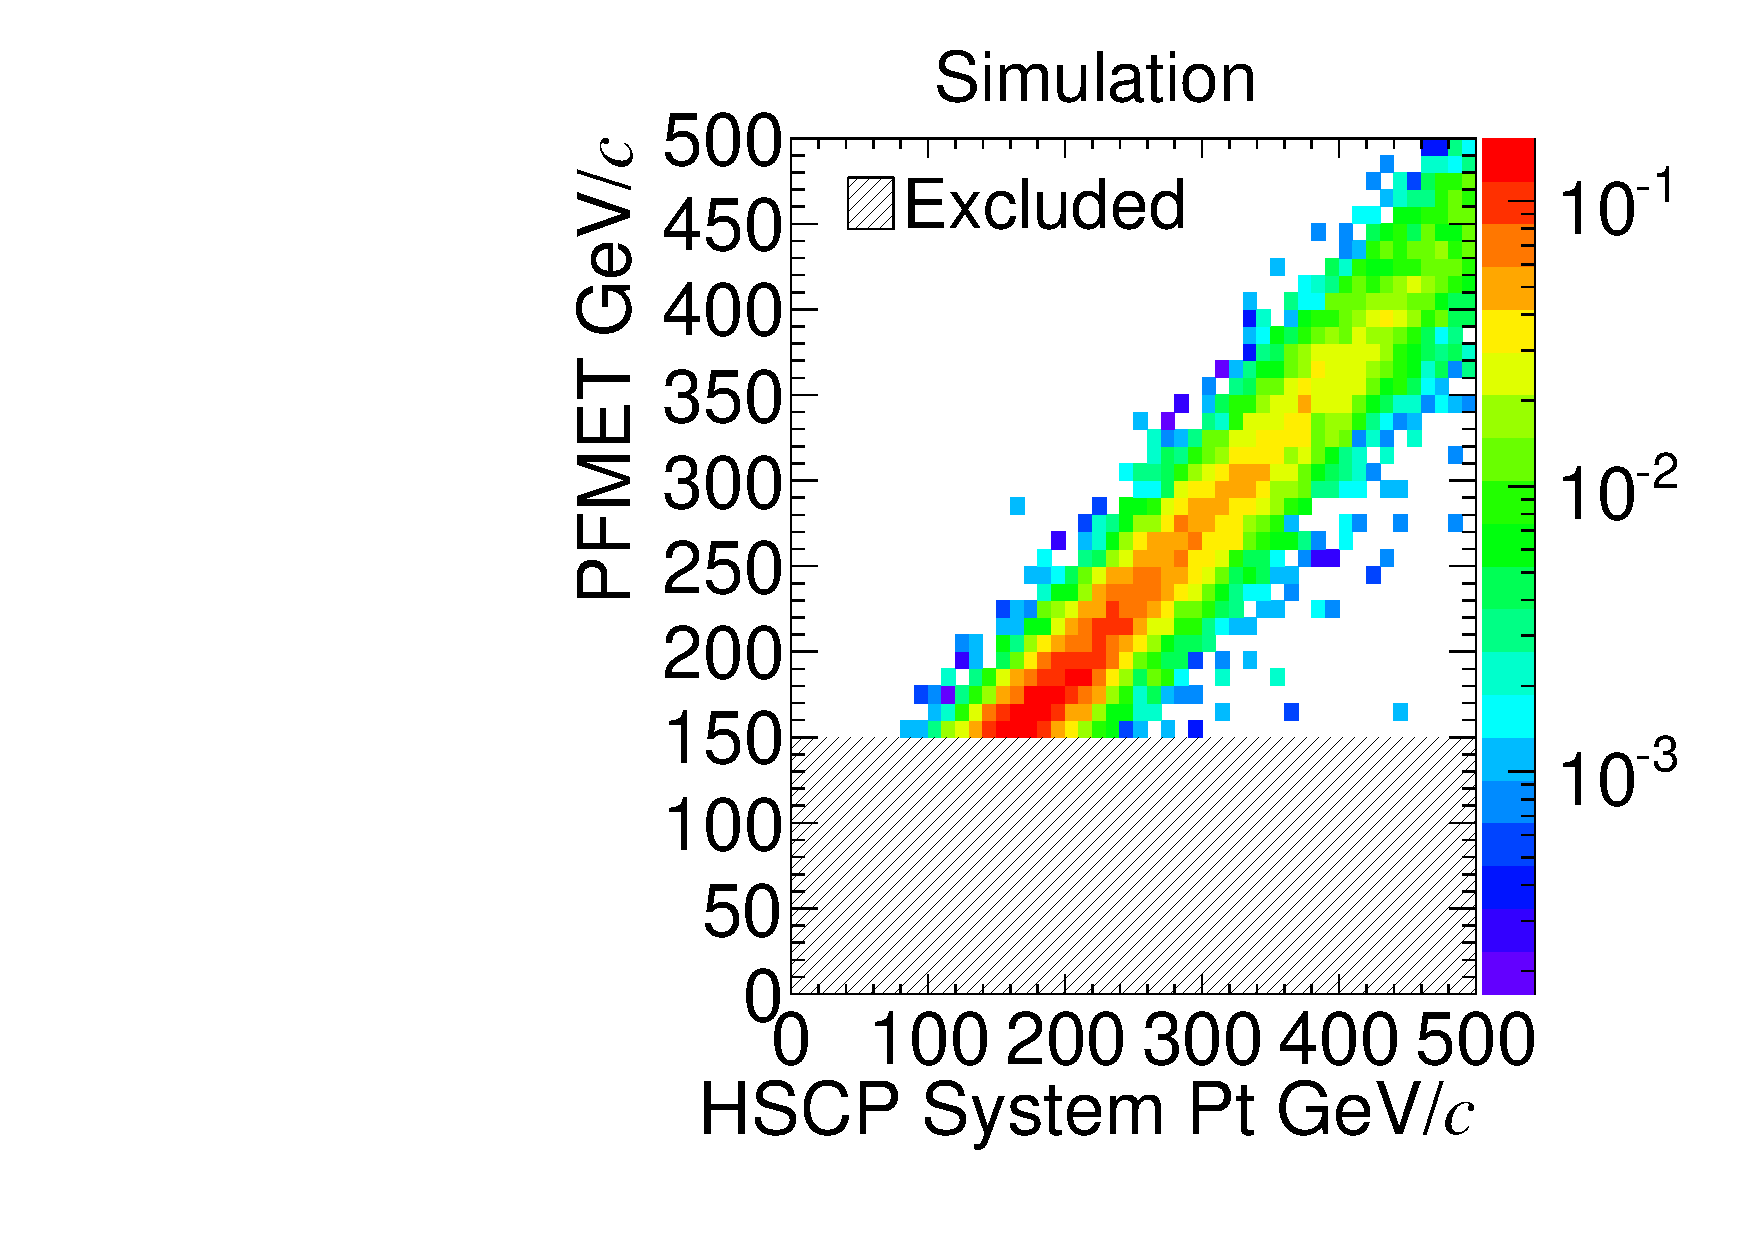
\includegraphics[clip=true, trim=0.0cm 0cm 3.0cm 0cm, width=0.44\textwidth]{figures/search/Gluino_8TeV_M1200N_f10SystPtMET} \\
      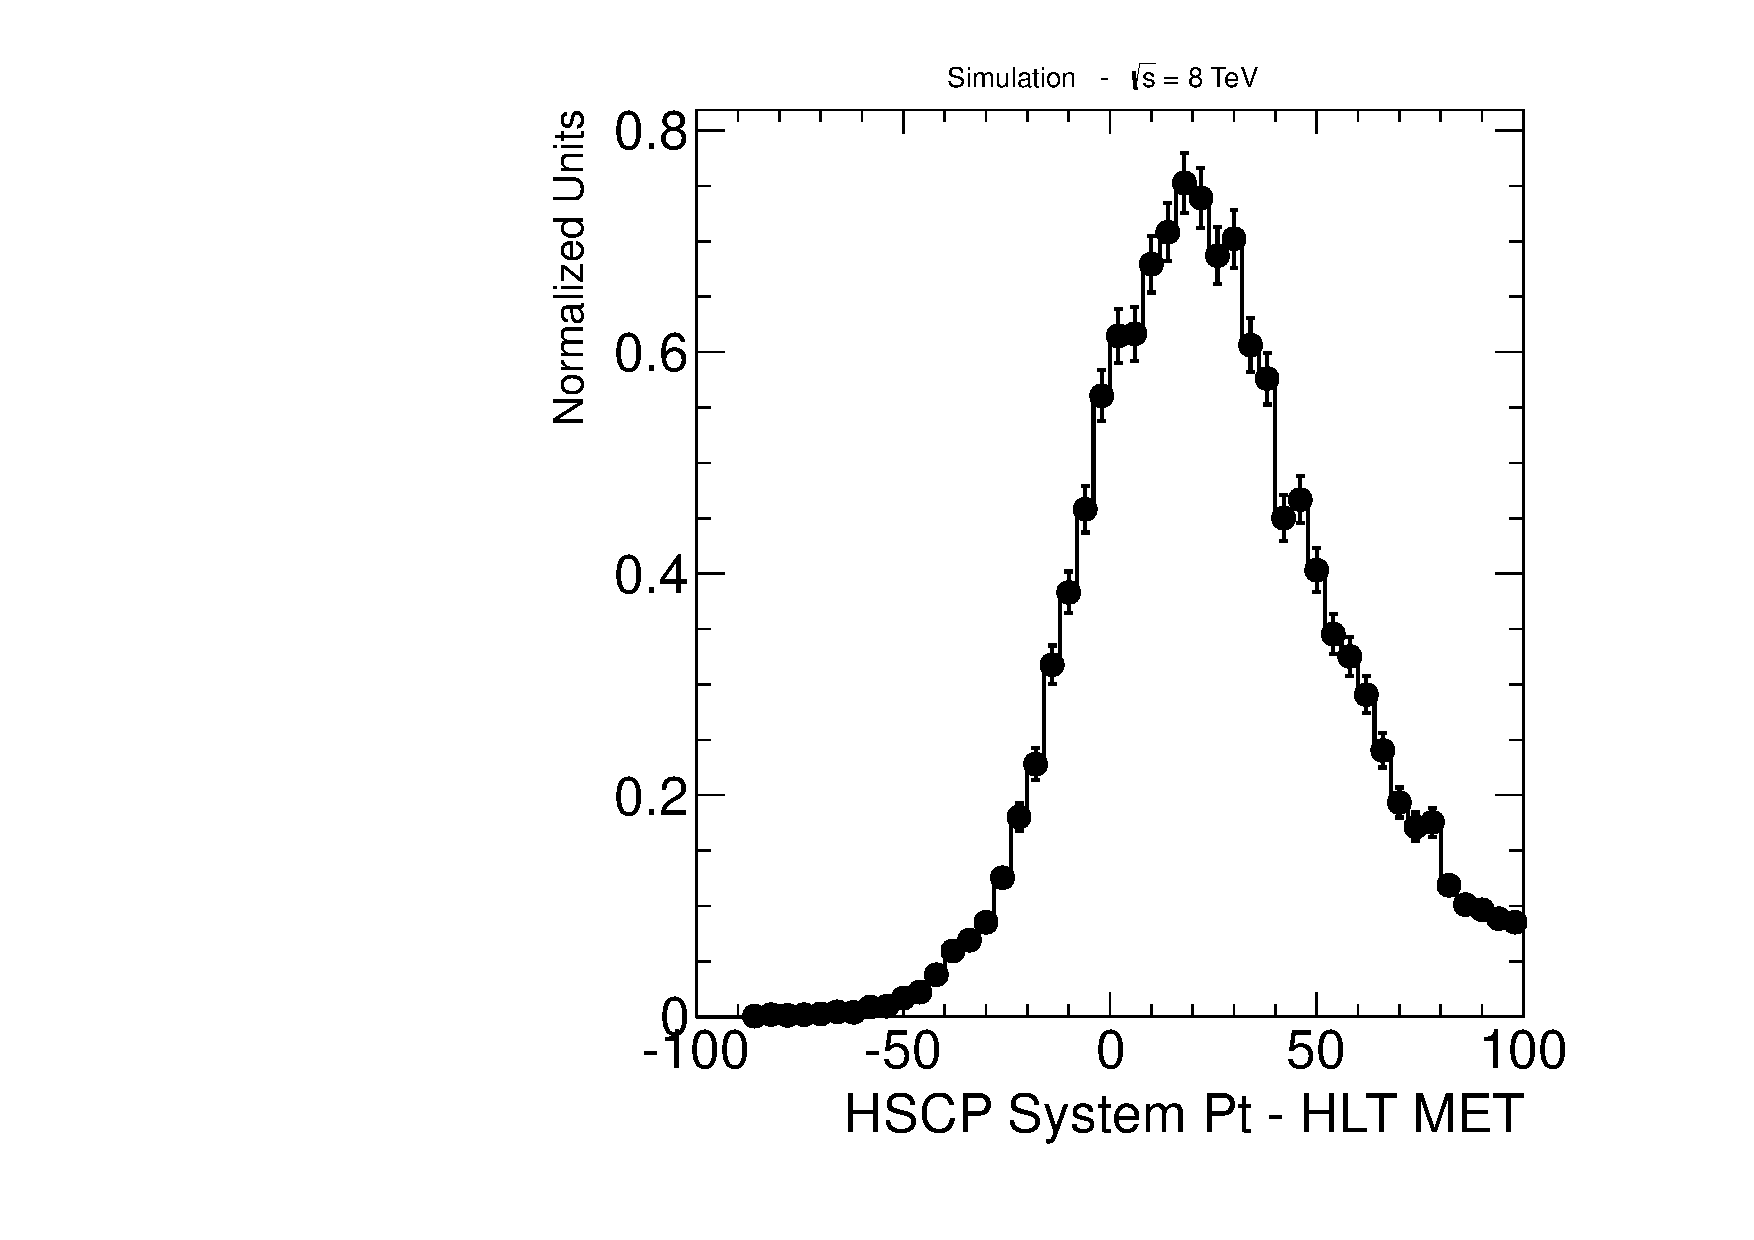
\includegraphics[clip=true, trim=0.0cm 0cm 3.0cm 0cm, width=0.44\textwidth]{figures/search/Gluino_8TeV_M1200N_f10SystPtDiffMET}
      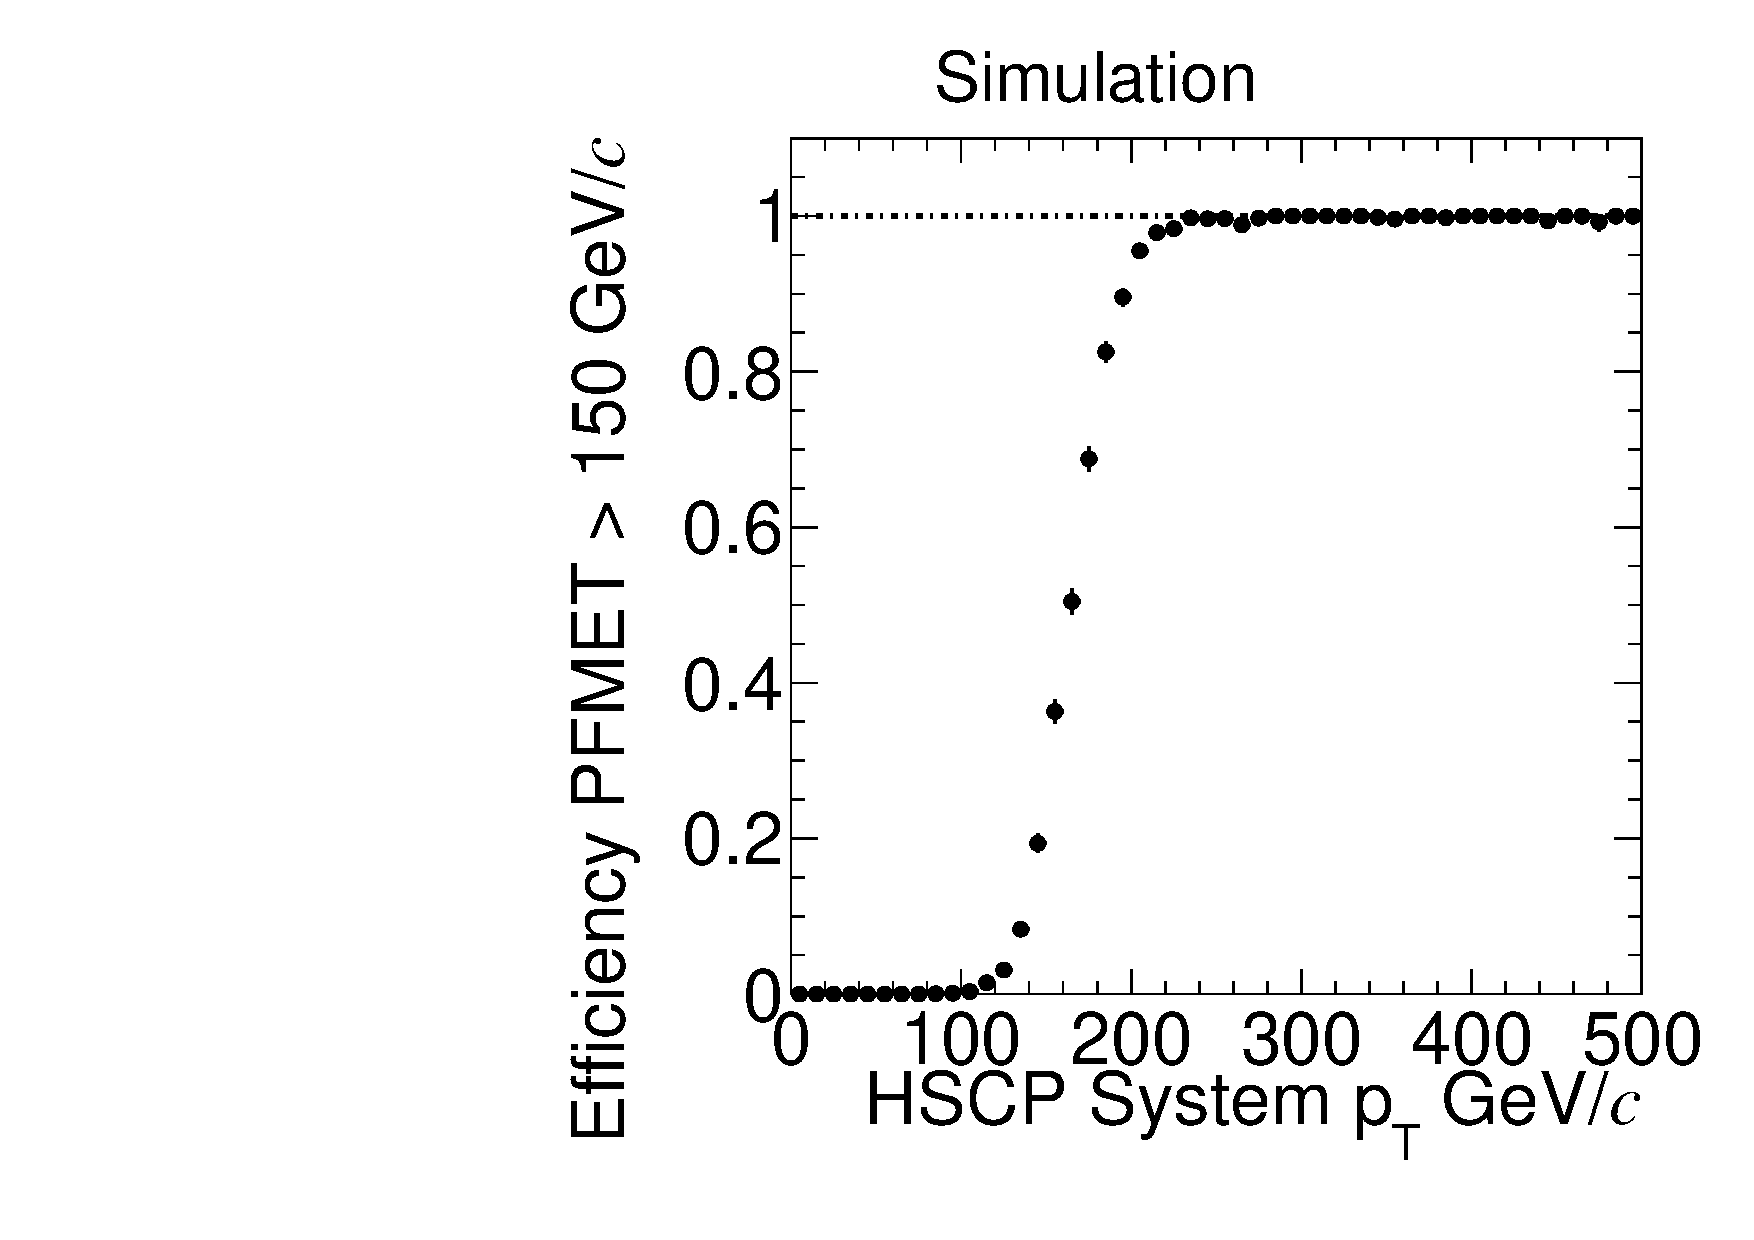
\includegraphics[clip=true, trim=0.0cm 0cm 3.0cm 0cm, width=0.44\textwidth]{figures/search/Gluino_8TeV_M1200N_f10SystPtEff}
      \caption[Comparison of di-HSCP system $\phi$ and \pt\ with online PFMET for a 1200~GeV
Gluino $f=0.1$ charge suppressed sample in events with at least 150~GeV of online PFMET]
      {Same as Fig.~\ref{fig:SystPtTrigger} but the sample used is 1200~GeV $f=0.1$ charge suppressed gluino.
%Comparison of di-HSCP system with online PFMET for a charge suppressed 1200 GeV Gluino $f=0.1$ sample in events with at least 150 GeV of online PFMET.
%         Top Left: Online PFMET $\phi$ versus di-HSCP system $\phi.$ Top Right: Online PFMET value versus di-HSCP system $p_T$.
%         Bottom Left: Difference between di-HSCP system $p_T$ and online PFMET value.
%         Bottom Right: Probability to have online PFMET greater than 150 versus di-HSCP system $p_T$.
        }
      \label{fig:SystPtTriggerN}
  \end{center}
\end{figure}

One trigger issue unique to slow-moving particles is the timing acceptance of the L1 trigger. If an HSCP arrives in the muon system too late it can trigger the
readout of the wrong bunch crossing window. As most of the CMS subdetectors, though not the muon system, are designed to not readout data coming from adjacent bunch crossing windows,
the data from the correct bunch crossing window would be lost. To help deal with this, members of the CMS L1 trigger team developed a special configuration of the
RPC L1 trigger to partially recover HSCP that arrive in the muon system in the bunch crossing window following the crossing that produced them.
This configuration is discussed in Sec.~\ref{sec:computing}

%The configuration creates a duplicate copy of all RPC hits and sends them to the muon trigger in the bunch crossing immediately preceding the arrival of the hits. 
%This allows for HSCP that
%arrive in the RPCs 0.5 -- 1.5 bunch crossings later than a collision muon would to still trigger the readout of the correct event. For particles that arrive in the RPC
%in the correct bunch crossing, a coincidence with the LHC beam crossing through CMS is required to prevent the readout of the previous event. This configuration
%was possible for 2012 running as the proton bunches were separated by 50ns despite having 25ns wide bunch crossing window windows.
%The configuration is described in more detail in Sec.~\ref{sec:computing}.

The first of the three algorithms used requires both a track to be found in the muon system with $p_T > 70$~GeV, $|\eta| < 2.1$, with at least two
muon stations associated with the track as well as PFMET $ > 55$~GeV. 
For the first 700 pb$^{-1}$ of 2012 running the threshold on PFMET was at 65~GeV. The signal samples are weighted
to account for the amount of data taken at each threshold. Events collected with this trigger are only used
in the \muononly\ analysis.
The second algorithm requires a track matched in both the inner tracker
and muon system to be found by the HLT with $p_T > 40$~GeV and $|\eta| < 2.1$. The only requirement for the third algorithm is PFMET $ > 150$~GeV.
The second and third algorithms are used in all the analyses.

The decision to use the pure PFMET trigger even when a muon signature is required offline is prompted by the late arrival of the HSCPs in the muon system.
Even with the RPC configuration described above, very slow moving HSCP can trigger the readout of the wrong event but still be reconstructed offline
if the event has been triggered by the pure PFMET trigger. This can be seen in Figure~\ref{fig:TriggerEffVsBetaGl} which shows the trigger efficiency versus $\beta$
with and without the pure PFMET trigger.
It can be seen that using the pure PFMET trigger allows the search to probe lower $\beta$ particles. 

%Additional triggers were developed to collect - Maybe add dE/dx triggers?

%As color charged $R$-hadron can be neutral
%while traversing CMS or arrive so late to the muon system that they are not able to be reconstructed offline an effective detector acceptance is defined 
%that at least one HSCP be reconstructed offline. Thus Figure~\ref{fig:TriggerEffVsBetaGl} shows the efficiency requiring an HSCP be reconstructed as a track
%as in the \muononly\ analysis, and as a global track, as in the the \tktof\ analysis.

\begin{figure}
\centering
%  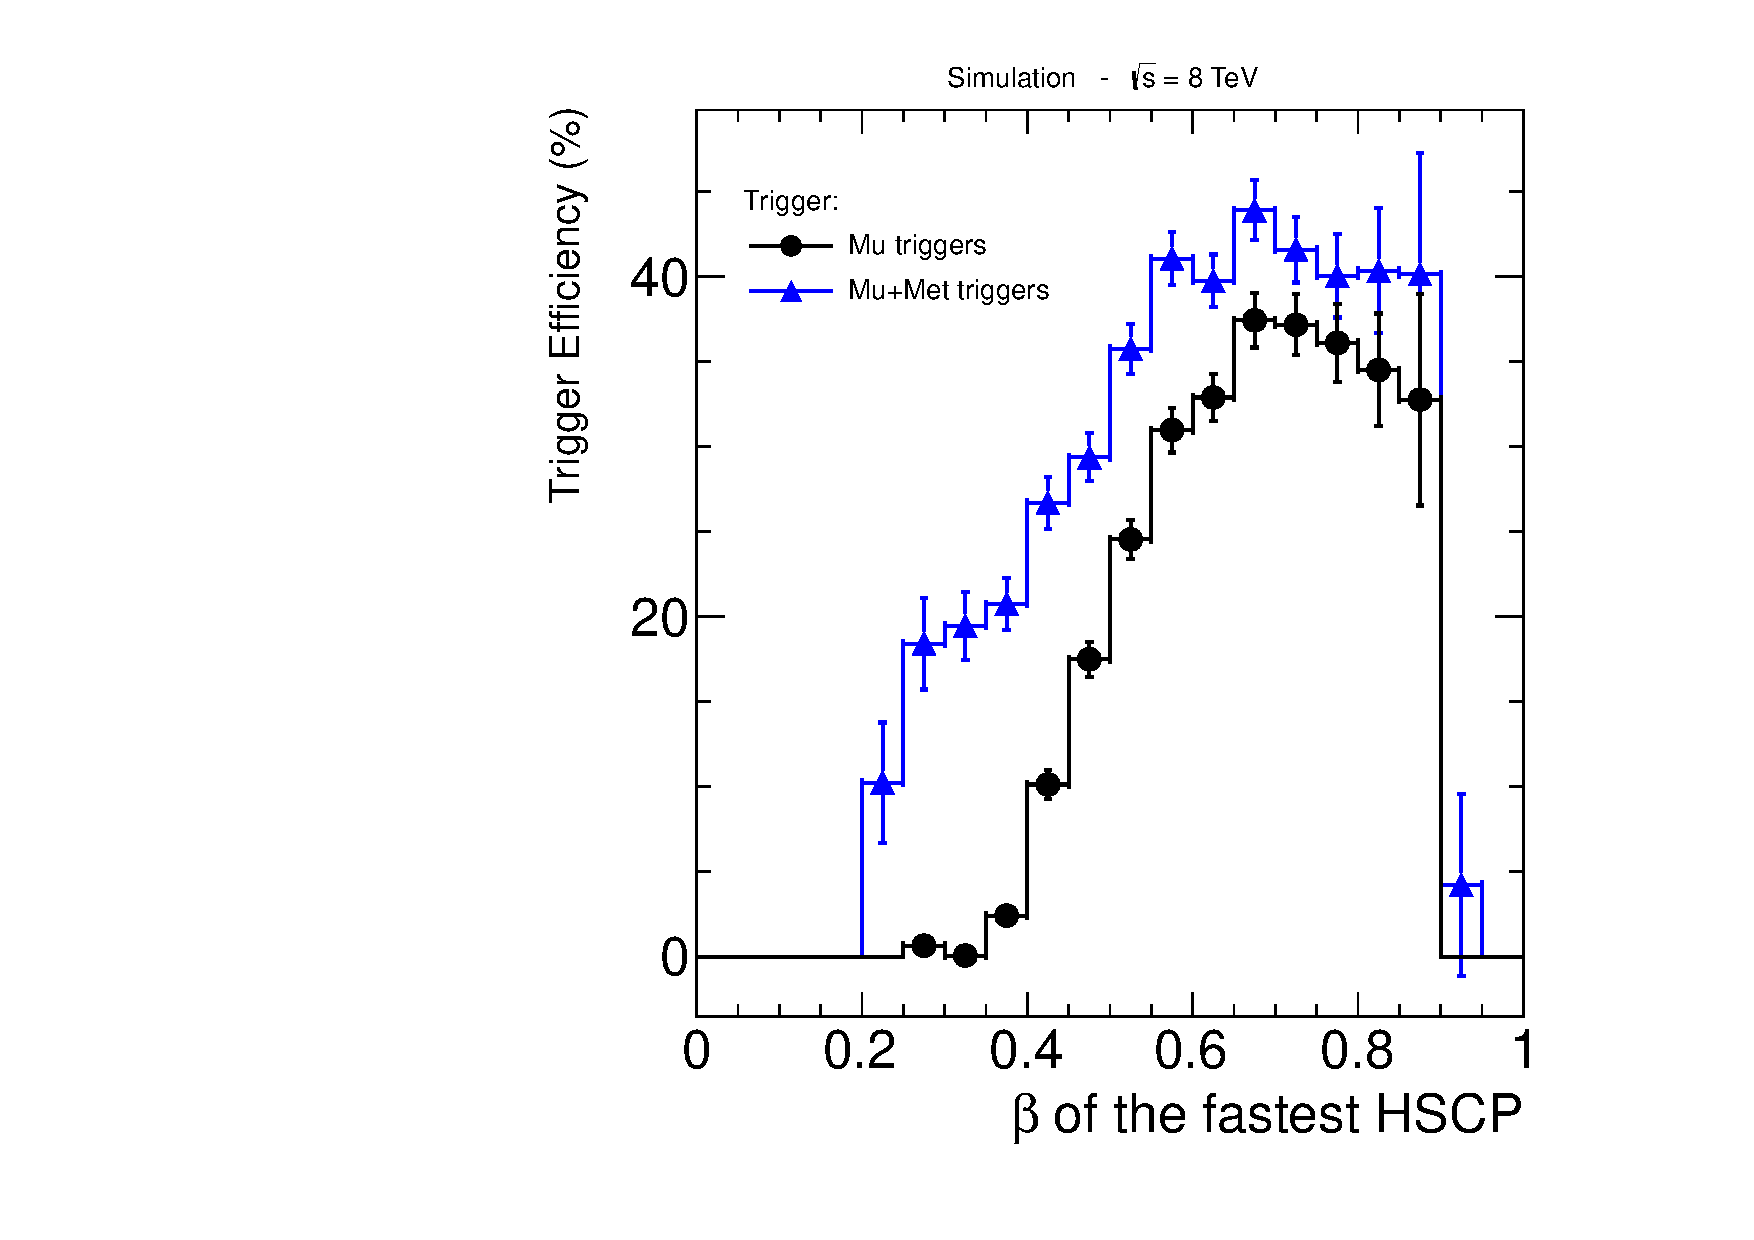
\includegraphics[clip=true, trim=0.0cm 0cm 3.0cm 0cm, width=0.44\textwidth]{figures/search/Gluino_8TeV_M1200_f100MatchedSA}
  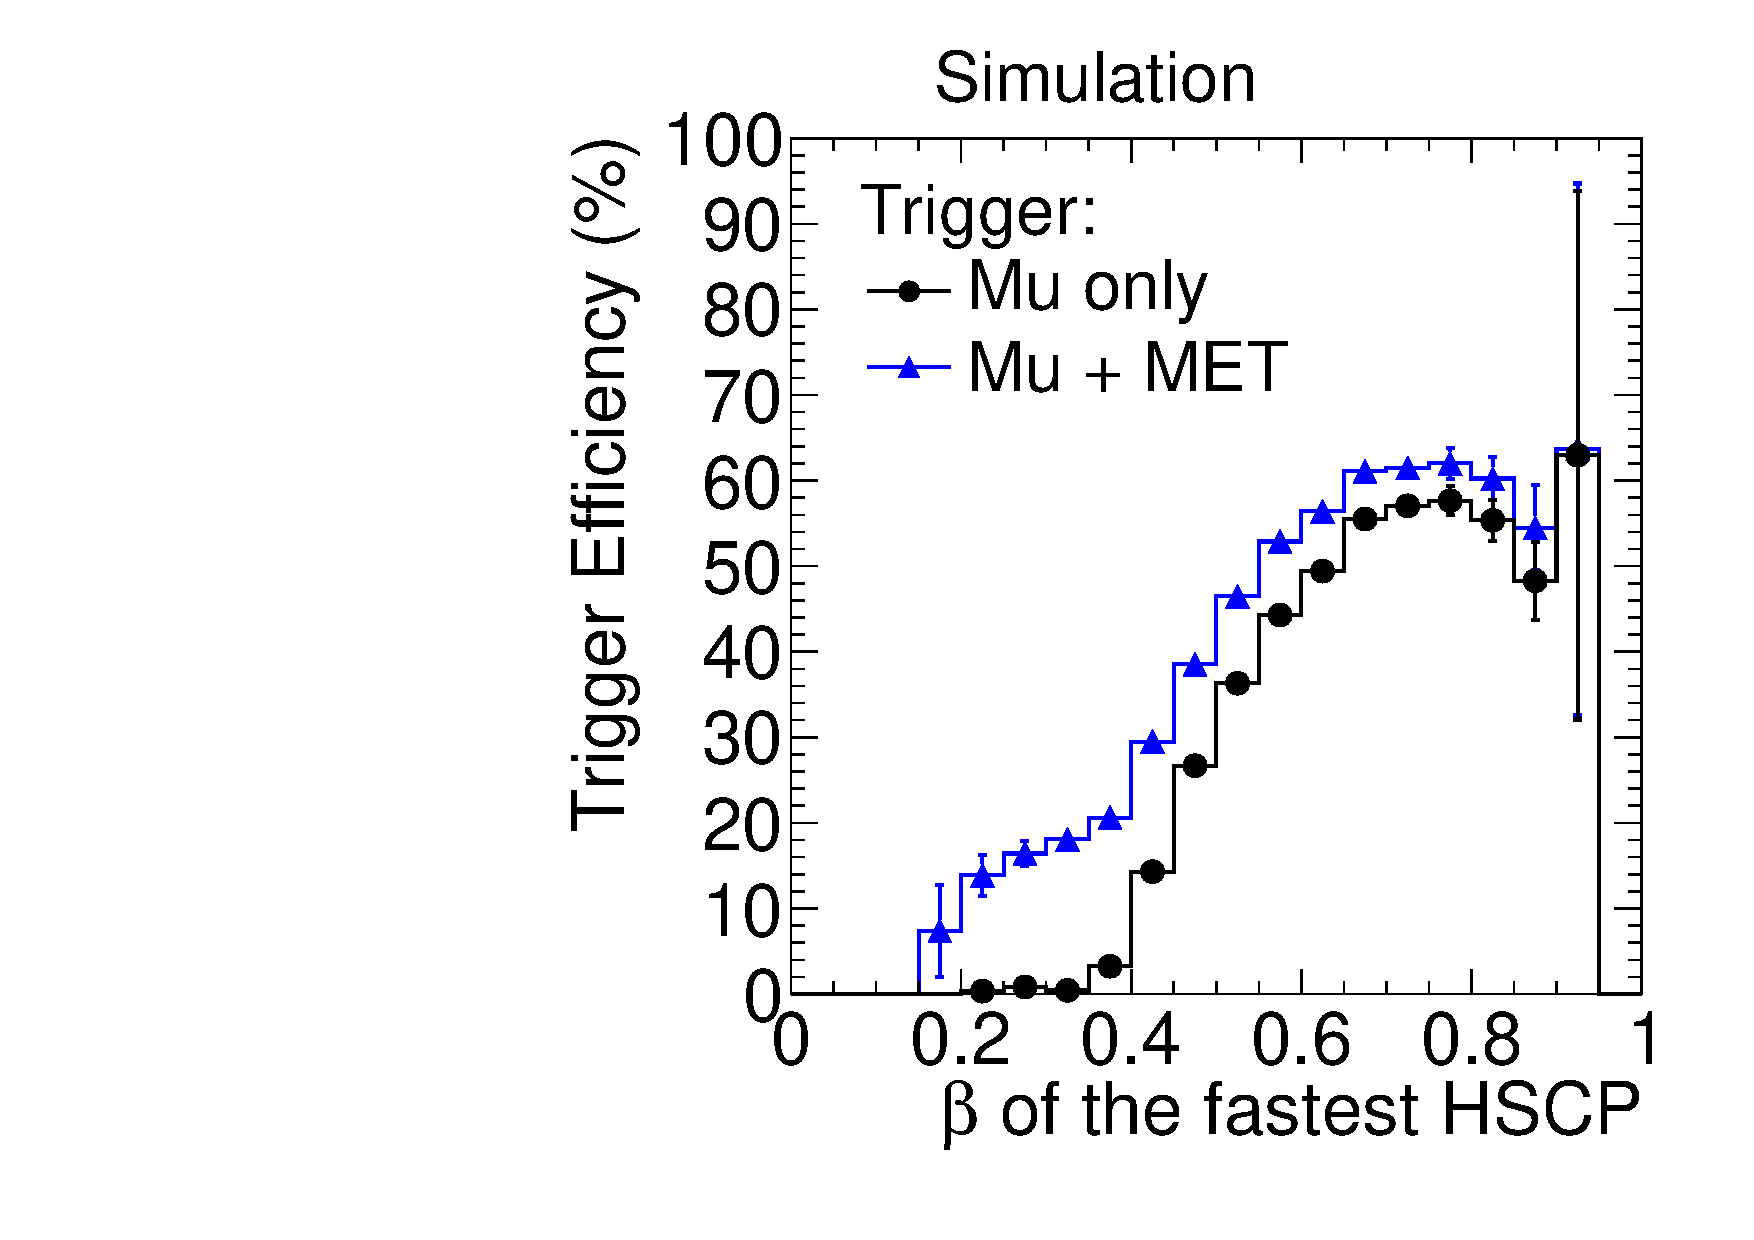
\includegraphics[clip=true, trim=0.0cm 0cm 3.0cm 0cm, width=0.44\textwidth]{figures/search/Gluino_8TeV_M1200_f10MatchedSA}
  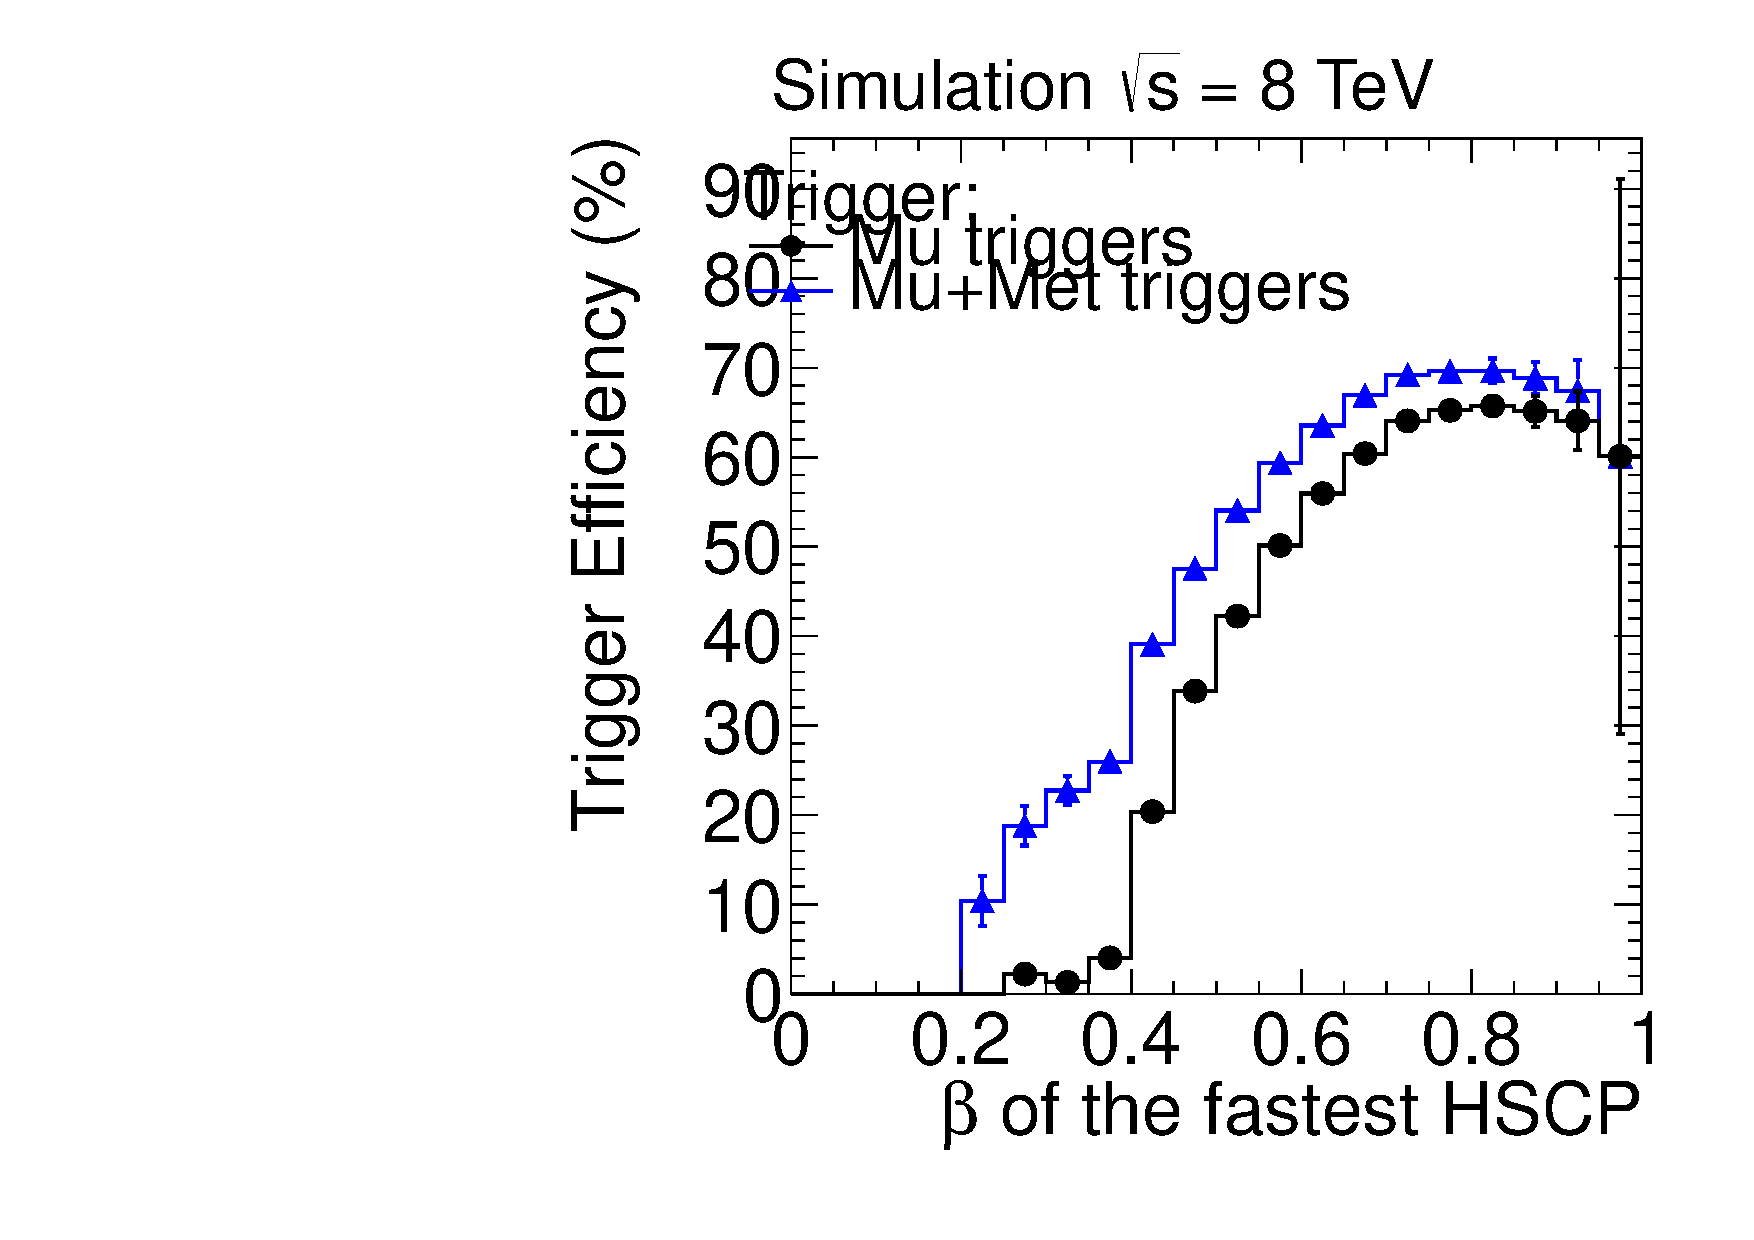
\includegraphics[clip=true, trim=0.0cm 0cm 3.0cm 0cm, width=0.44\textwidth]{figures/search/Stop_8TeV_M800MatchedSA}
%  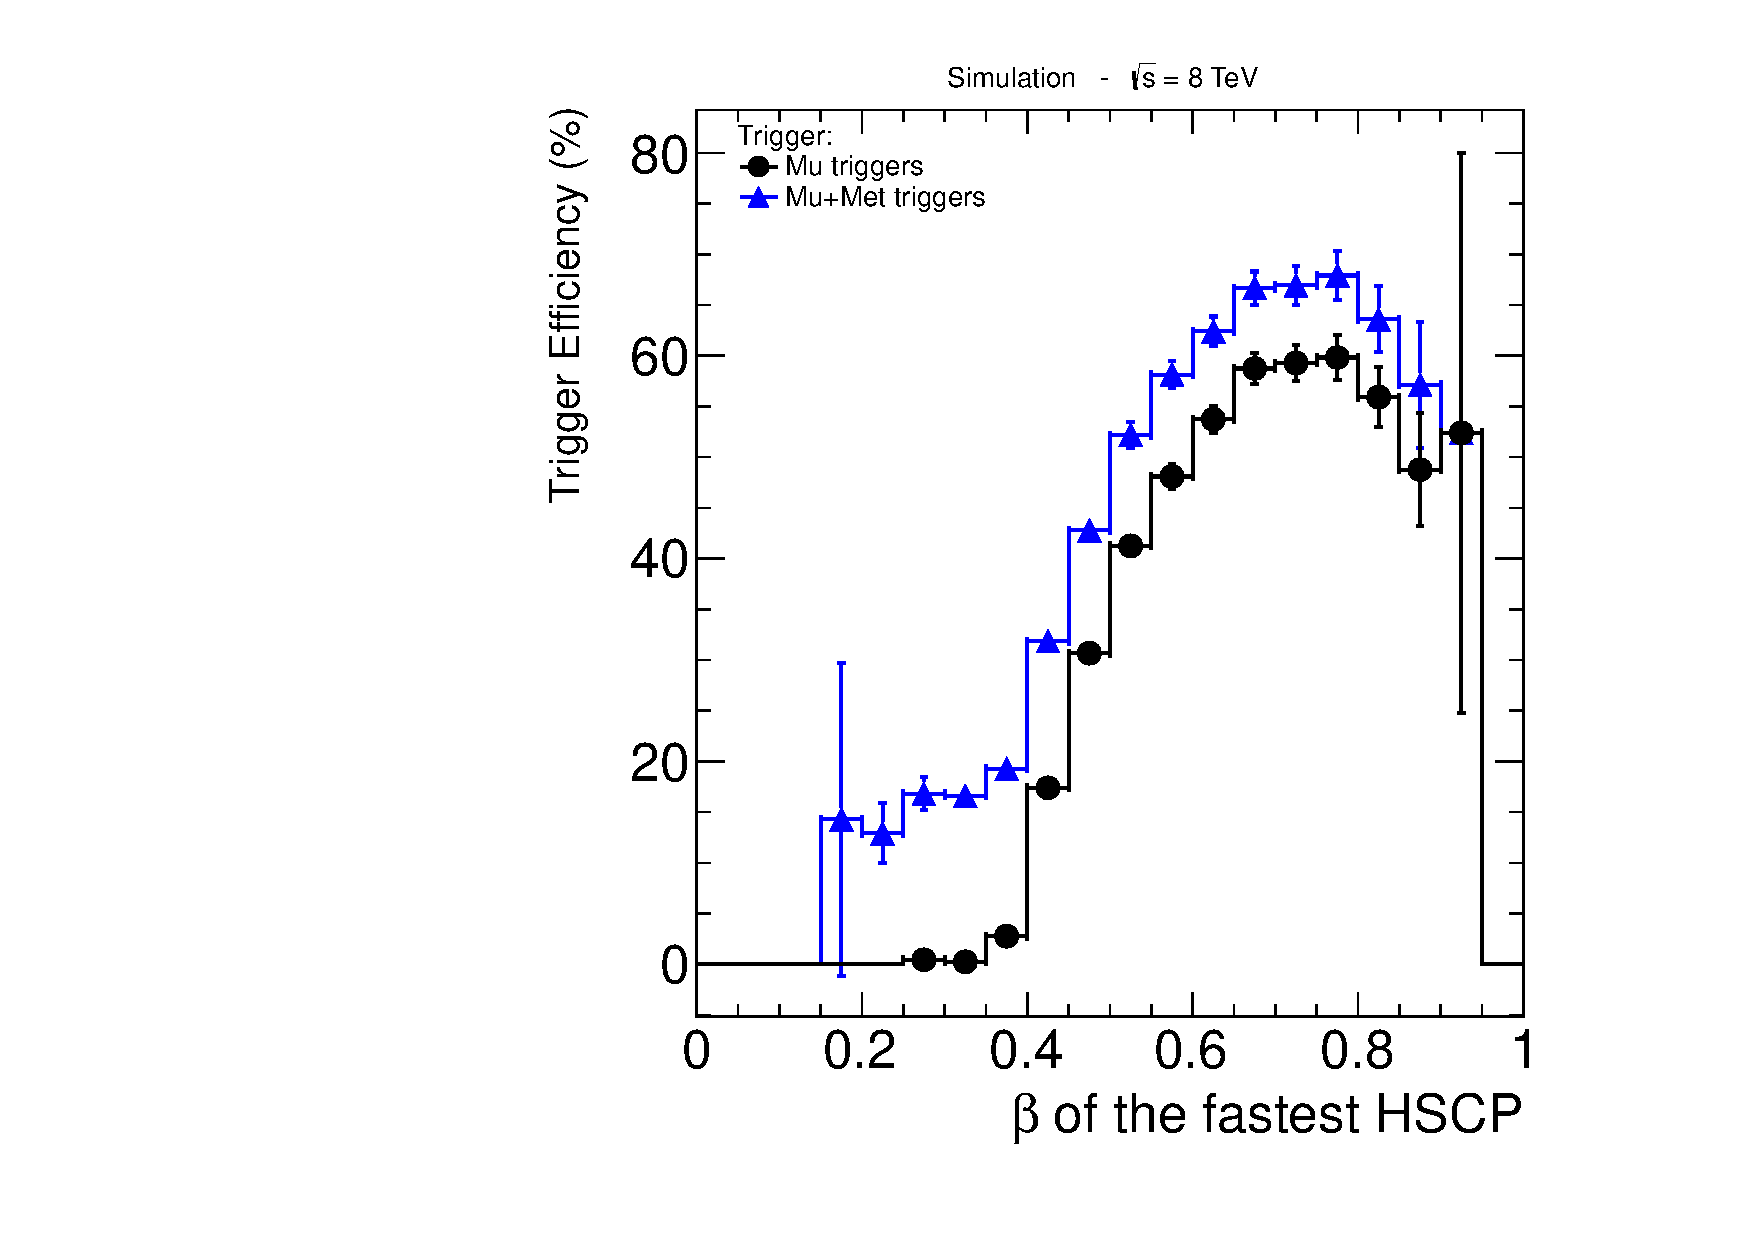
\includegraphics[clip=true, trim=0.0cm 0cm 3.0cm 0cm, width=0.32\textwidth]{figures/search/Gluino_8TeV_M1200_f10MatchedGl}
%  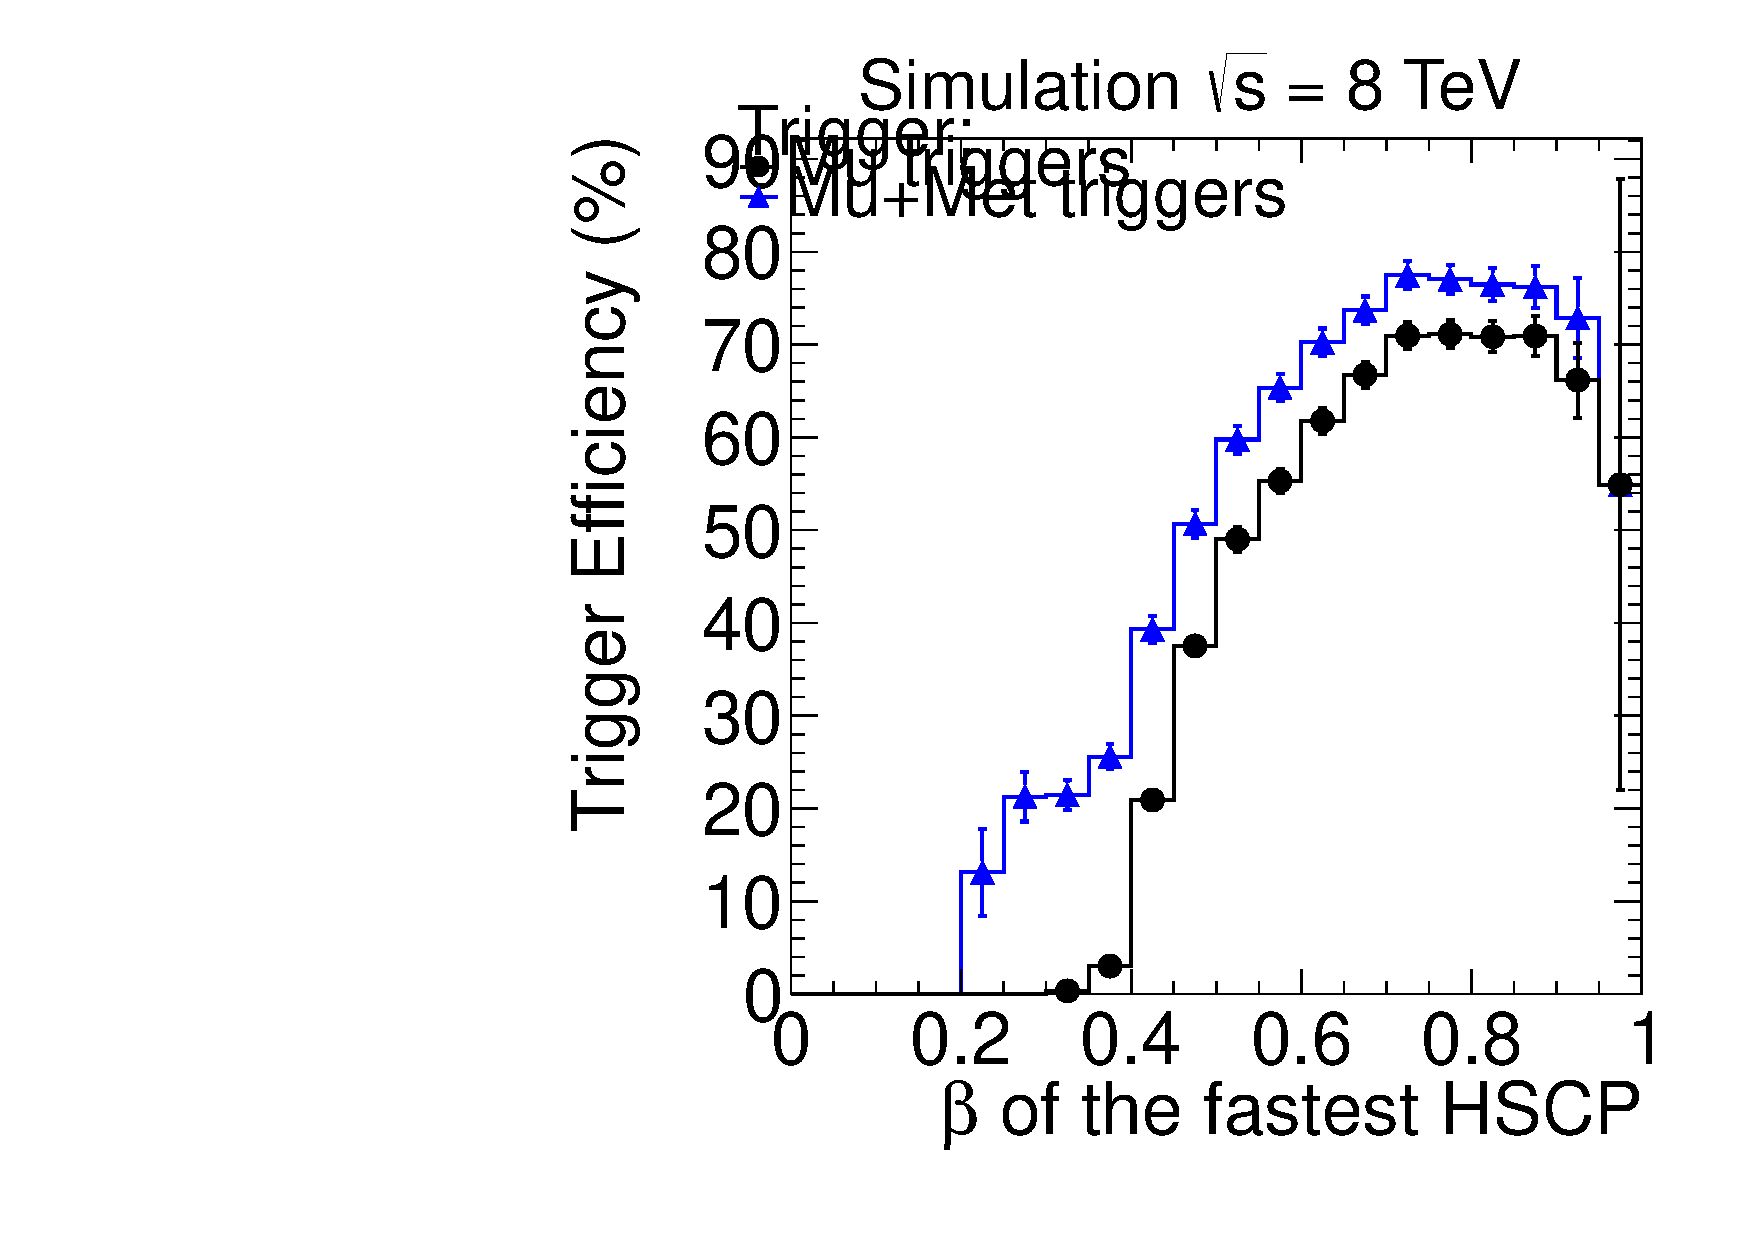
\includegraphics[clip=true, trim=0.0cm 0cm 3.0cm 0cm, width=0.32\textwidth]{figures/search/Stop_8TeV_M800MatchedGl}
%  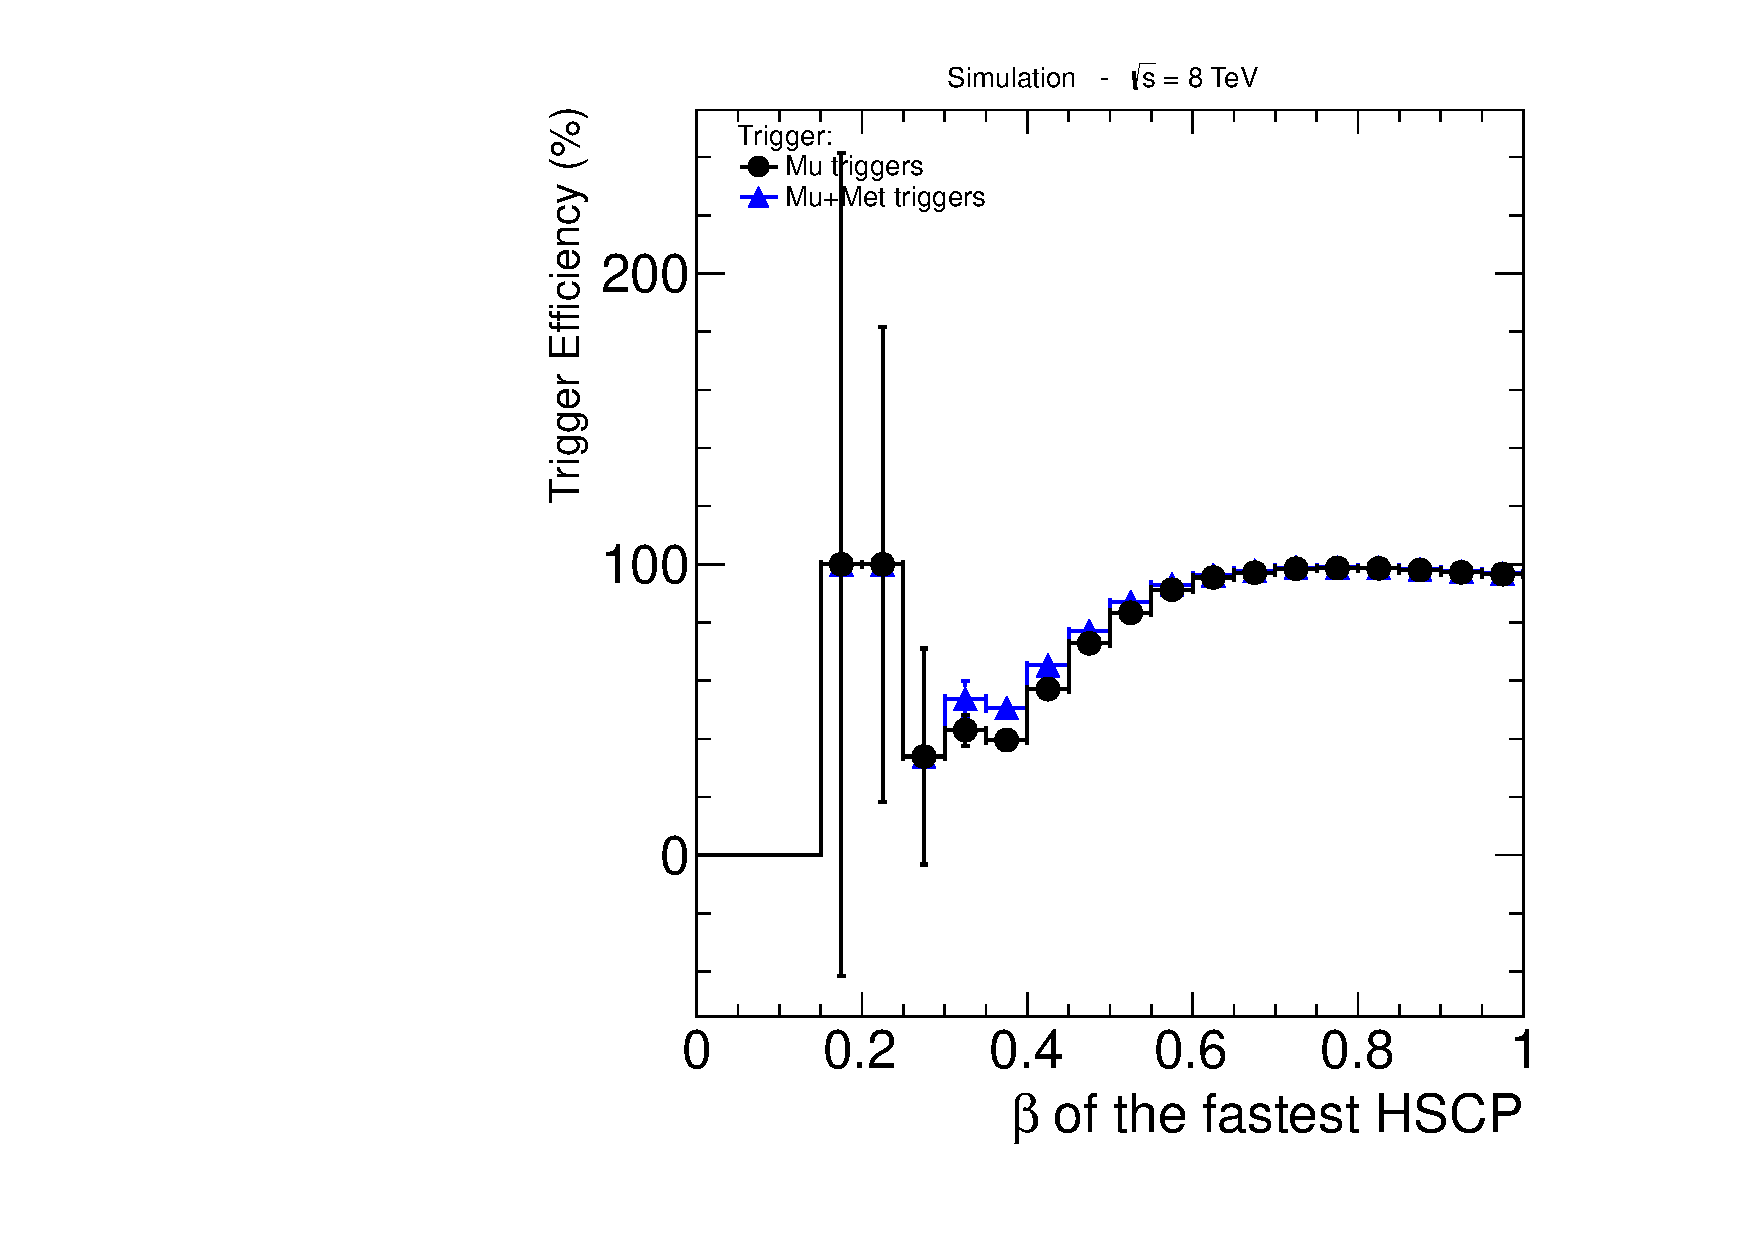
\includegraphics[clip=true, trim=0.0cm 0cm 3.0cm 0cm, width=0.32\textwidth]{figures/search/GMStau_8TeV_M494MatchedGl}
      \caption[Trigger efficiency as a function of the $\beta$ of the fastest HSCP reconstructed offline in the muon system with only the muon triggers
and additionally including the PFMET trigger.]
{Trigger efficiency as a function of the $\beta$ of the fastest HSCP reconstructed offline in the muon system with only the muon triggers
and additionally including the PFMET trigger.
Sample is 1200~GeV Gluino $f=0.1$ (left) and 800~GeV stop (right)}
    \label{fig:TriggerEffVsBetaGl}
\end{figure}

When evaluating trigger efficiencies, it is important to only consider events that have a possibility of being selected offline.
For the case of strongly charged HSCP this is made more difficult as some events may not have any $R-hadrons$ electrically charged while they pass through the detector.
To deal with this, the trigger efficiencies are reported with respect to events where at least one HSCP is found offline.
The efficiency for each trigger as well as the combined efficiency is listed for various signals in Tables~\ref{tab:triggEffSA} and ~\ref{tab:triggEffGl} in events
with at least one HSCP reconstructed in the muon system and muon system plus tracker, respectively.

\begin{table}
 \begin{center}
  \caption[Trigger efficiency for various models considered with respect to events with a reconstructed HSCP in the muon system]
{Trigger efficiency for various models considered using the SingleMu, PFMET, L2Mu+MET or a combination of the three.
Efficiencies with respect to events with at least one HSCP reconstructed in the muon system.}
     \label{tab:triggEffSA}
  \begin{tabular}{|l|c|c|c|c|c|} \hline
      Model     & Mass (GeV) & Mu40       & PFMET150   &  L2Mu+MET  & Total                 \\ \hline
 Gluino $f=0.1$ &  400  & 35.55      & 19.41      & 34.28      & 58.56    \\
 Gluino $f=0.1$ &  800  & 31.63      & 22.57      & 31.21      & 54.88    \\
 Gluino $f=0.1$ & 1200  & 26.62      & 20.45      & 24.63      & 47.52    \\
 Gluino $f=1.0$ &  400  &  5.55      & 23.22      & 36.63      & 46.07    \\
 Gluino $f=1.0$ &  800  &  5.01      & 24.50      & 31.88      & 43.41    \\
 Gluino $f=1.0$ & 1200  &  3.69      & 20.62      & 23.62      & 35.45    \\
           Stop &  200  & 42.79      & 11.15      & 27.31      & 58.80    \\
           Stop &  500  & 42.07      & 19.79      & 31.13      & 61.21    \\
           Stop &  800  & 41.57      & 21.57      & 30.33      & 60.73    \\ \hline
  \end{tabular}
 \end{center}
\end{table}

\begin{table}
 \begin{center}
      \caption[Trigger efficiency for various models considered with respect to events with a reconstructed HSCP in both the muon system and inner tracker]
{Trigger efficiency for various models considered using the SingleMu, PFMET, or a combination of the two.
Efficiencies with respect to events with at least one HSCP reconstructed in both the muon system and inner tracker.}
     \label{tab:triggEffGl}
  \begin{tabular}{|l|c|c|c|c|} \hline
      Model     & Mass (GeV) & Mu40       & PFMET150   & Total                 \\ \hline
 Gluino $f=0.1$ &  400  & 51.87      & 16.06      & 59.09    \\
 Gluino $f=0.1$ &  800  & 46.50      & 20.50      & 56.42    \\
 Gluino $f=0.1$ & 1200  & 38.96      & 19.56      & 49.95    \\
 Gluino $f=1.0$ &  400  & 41.81      & 19.36      & 51.76    \\
 Gluino $f=1.0$ &  800  & 37.83      & 21.57      & 49.01    \\
 Gluino $f=1.0$ & 1200  & 31.70      & 21.16      & 45.21    \\
           Stop &  200  & 58.43      &  7.69      & 61.54    \\
           Stop &  500  & 56.91      & 17.40      & 64.44    \\
           Stop &  800  & 56.15      & 20.49      & 65.59    \\
      GMSB Stau &  100  & 97.86      & 14.74      & 98.06    \\
      GMSB Stau &  308  & 97.03      & 17.53      & 97.47    \\
      GMSB Stau &  494  & 95.56      & 17.76      & 96.35    \\
        PP Stau &  100  & 95.06      &  0.17      & 95.09    \\
        PP Stau &  200  & 95.78      &  0.37      & 95.82    \\
        PP Stau &  494  & 95.23      &  1.16      & 95.36    \\ \hline
  \end{tabular}
 \end{center}
\end{table}

Muons from cosmic rays are an important background for the \muononly\ analysis. To study and predict them a trigger that selects events when no beams are passing through
CMS is used. The trigger requires the presence of a muon system track with $p_T > 20$~GeV, no proton bunches passing through CMS within 50ns, and for the event not to be flagged as
noise from the LHC beams. The muon system track reconstruction used for the cosmic ray muon trigger is slightly 
different than for the collision trigger as it is not updated at vertex,
the meaning of this is discussed in section~\ref{sec:preselection}. However, both reconstructions are required offline so no bias is introduced.